% !TEX root = ./notes.tex
\chapter{Notes on nuclear physics}
\newcommand{\rn}{\ensuremath{r_{\mathrm{N}}}}
\newcommand{\re}{\ensuremath{r_{\mathrm{E}}}}
\newcommand{\barn}{\ensuremath{\mathrm{b}}}
\newcommand{\EG}{\ensuremath{E_{\mathrm{G}}}}
\newcommand{\Epk}{\ensuremath{E_{\mathrm{pk}}}}

\section{The Nuclear Landscape}

From nucleon-nucleon scattering, we find that the nuclear force operates over a range of $\lesssim 2\ee{-13}\nsp\cm = 2\nsp\fermi$.  It is attractive over this range, but is repulsive at distances $< 1\nsp\fermi$.  In this aspect, the interaction resembles the interaction between molecules in a fluid.  Indeed, for heavy nuclei, the nucleons form ``nuclear matter'' with a characteristic density of $0.16\nsp\fermi^{-3}$ and a binding energy of $\approx 8\nsp\MeV$.  Here the \emph{binding energy} is defined as
\begin{equation}\label{e.binding-energy-def}
B(N,Z) = Z m_{p} + N m_{n} - M(N,Z),
\end{equation}
where $M$ is the total mass of a nucleus with $N$ neutrons and $Z$ protons. The fact that the nuclear interaction binds the nucleons into a ``nuclear matter'' means that one can make a crude model of the nucleus as a liquid drop, and fit this formula to experimental masses.  This model, due to Weiz\"acker, is
\begin{equation}\label{e.weizacker-fmla}
-B(N, Z) = a_{V} A + a_{S}A^{2/3} + a_{A}\frac{(N-Z)^{2}}{A} + a_{C}\frac{Z^{2}}{A^{1/3}}.
\end{equation}
Here $A = N+Z$ and masses are in MeV, so $m_{p} = 938.272\nsp\MeV$ and $m_{n} = 939.565\nsp\MeV$. Using the online fitting routine from the \href{http://128.95.95.61/~intuser/ld.html}{Institute for Nuclear Theory}, I obtained the following coefficients.

\begin{table}[htbp]
\caption{Coefficients for the Weiz\"acker mass formula.\label{t.liquid-drop-coefficients}}
\centering
\begin{tabular}{l|rrrr}
\hline
coefficient & $a_{V}$ & $a_{S}$ & $a_{A}$ & $a_{C}$\\
\hline\hline
value (MeV) & -15.5 & 16.6 & 22.7 & 0.71\\
\hline
\end{tabular}
\end{table}

This simple formula contains a good description of the nuclear landscape.  First, let us look at the binding energy per nucleon, $-B/A$.  Dividing equation~(\ref{e.weizacker-fmla}) by $A$, and denoting the neutron asymmetry by $\eta \equiv (N-Z)/(N+Z)$, we obtain
\[ -\frac{B}{A} = a_{V} + a_{S} A^{-1/3} + a_{A}\eta^{2} + \frac{a_{C}}{4} \left( 1-2\eta\right)^{2} A^{2/3}. \]
For small $A$, we see that the most bound nuclei have $eta = 0$, i.e., equal numbers of neutrons and protons.  As $A$ increases, however, the Coulomb term becomes important.  Expanding the last two terms and combining, we have the sum of the asymmetry and Coulomb terms,
\[ \frac{a_{C}}{4} A^{2/3} - a_{C}A^{2/3}\eta + \left[ a_{C}A^{2/3} + a_{A} \right] \eta^{2} .\]
For large $A$, this expression is minimized (although it cannot be made to vanish) for $\eta < 0$: that is, $N>Z$ and the most bound massive nuclei are neutron-rich. The nuclei for which $-B/A$ is a minimum for a fixed $A$ define the \emph{valley of stability}. How does the binding energy change with $A$ along this valley?  At small $A$, the asymmetry term dominates and $\eta^{2}\ll 1$.  As $A$ increases, the surface term $a_{S}A^{-1/3}$ becomes smaller and $B/A$ increases.  At large $A$, however, the sum of the Coulomb and asymmetry terms decreases $B/A$.  As a result, there is a peak in $B/A$, which is around $A\approx 56$.

Define the \emph{neutron separation energy} $S_{n}$ as the energy needed to remove a neutron from a nucleus,
\begin{eqnarray}\label{e.Sn}
S_{n}(N,Z) &\equiv& \left[M(N-1,Z) + m_{n}\right] - M(N,Z) \nonumber\\
	&=& B(N,Z) - B(N-1,Z).
\end{eqnarray}
Likewise, define the \emph{proton separation energy} as
\begin{eqnarray}\label{e.Sp}
S_{p}(N,Z) &\equiv& \left[M(N,Z-1) + m_{p}\right] - M(N,Z) \nonumber\\
	&=& B(N,Z) - B(N,Z-1).
\end{eqnarray}
If we take a nucleus $(N,Z)$ in the valley of stability and add protons keeping $N$ fixed, we will eventually reach a nucleus for which $S_{p} = 0$, that is, it costs no energy to add or remove a proton.  This defines the \emph{proton-drip line}: nuclei more proton-rich are unstable to proton emission. Likewise, on the neutron-rich side there is the \emph{neutron-drip line}, for which $S_{n} = 0$.

\section{Non-resonant nuclear reactions}

The situation we are interested in is the reaction between two nuclei, $(A_{1},Z_{1})$ and $(A_{2},Z_{2})$.  The nuclear radius is $\rn\approx A^{1/3 }\times 10^{-13}\nsp\cm = A^{1/3}\nsp\fermi$, and the Coulomb energy at this distance is
\begin{equation}\label{e.cb}
\frac{Z_{1}Z_{2}e^{2}}{\rn} = \frac{Z_{1}Z_{2}\alpha \hbar c}{ \rn} \approx 1.4 Z_{1}Z_{2}A^{-1/3}\nsp\MeV\gg kT.
\end{equation}
Here $\alpha = e^{2}/(\hbar c) = 1/137$ is the fine-structure constant and $\hbar c = 197 \nsp\MeV\usp\fermi$.  Remember these numbers!  If you want to impress your friends, you can do this in your head by remembering that $e^{2} = \alpha \hbar c = (197\nsp\MeV\usp\fermi)/137 = 1.44\nsp\MeV\usp\fermi = 1440\nsp\keV\usp\fermi$.  Clearly the cross-section for a reaction between our pair of particles is controlled by the probability of tunneling through the Coulomb potential.

For a two-body system, it is convenient to transform into a center-of-mass frame.  Our problem then reduces to a one-body problem with reduced mass $m = A\mb$, with $A=A_{1}A_{2}/(A_{1}+A_{2})$ and incident energy $E = m v^{2}/2$, where $v$ is the relative velocity of the two particles.  For now, we'll neglect angular momentum ($\ell = 0$) so our scattering is s-wave.
At low energies, we can form a ``geometrical'' cross-section from the particle wavenumber $k = p/\hbar$, with
\begin{equation}\label{e.geo}
\pi k^{-2} = \pi\frac{\hbar^{2}}{(2mE)^{1/2}} = 660\nsp\barn\frac{1}{A}\left(\frac{\keV}{E}\right)^{1/2}
\end{equation}
Here the cross-section is in units of \emph{barns}, with $1\nsp\barn = 10^{-24}\nsp\cm^{2}$.  This is the first part of our nuclear cross-section $\sigma(E)$. 

The second portion of the nuclear cross-section is the probability of tunneling through the Coulomb barrier.  First, let's get the classical turning point \re\ from
\begin{eqnarray}
\frac{Z_{1}Z_{2}e^{2}}{\re} &=& E,\nonumber\\
\re &=& 1440\nsp\fermi\nsp Z_{1}Z_{2}\left(\frac{\keV}{E}\right).
\end{eqnarray}
Now the wavelength is $k^{-1} = \hbar(2A\mb E)^{-1/2} = \hbar c (2A\mb c^{2} E)^{-1/2}$ and since $\mb c^{2} = 932\nsp\MeV$ the wavelength $k^{-1} = 145\nsp\fermi\usp(\keV/E)^{1/2}$. The important point is that since $k^{-1}\ll \re$, we can solve the Schr\"odinger equation using the WKB approximation.

The WKB approximation is standard, so let me just remind you that the probability of tunneling through the barrier depends on the \emph{action},
\begin{equation}\label{e.wkb}
\mathcal{P} \propto \exp\left\{\frac{2}{\hbar}\int_{\re}^{\rn}\left[2m\left(\frac{Z_{1}Z_{2}e^{2}}{r}-E\right) \right]^{1/2}\,\dif r\right\}.
\end{equation}
To do this integral, note that $\re\gg\rn$, so we can make the approximation $\rn\to 0$ and change variables to
\[
\sin\phi = \left[2m\left(\frac{Z_{1}Z_{2}e^{2}}{r}-E\right) \right]^{1/2}\frac{r}{2mZ_{1}Z_{2}e^{2}};
\]
with this substitution we tame the integral and obtain
\begin{equation}\label{e.prob}
\mathcal{P} \propto \exp\left\{-\frac{8mZ_{1}Z_{2}e^{2}}{\hbar(2mE)^{1/2}}\int_{0}^{\pi/2}\sin^{2}\phi\,\dif\phi\right\} = \exp\left[-\left(\frac{\EG}{E}\right)^{1/2}\right],
\end{equation}
where
\begin{equation}\label{e.EGamow}
\EG\equiv 2\pi^{2} A \mb c^{2} \alpha^{2} (Z_{1}Z_{2})^{2} = 979\nsp\keV \nsp A (Z_{1}Z_{2})^{2}
\end{equation}
is the \emph{Gamow energy}.  Note the strong dependence on $Z_{1}Z_{2}$: \EG\ determines which reactions can occur at a given temperature. If you stare at the factor multiplying the integral in equation~(\ref{e.prob}), you will see that $\mathcal{P}\propto \exp(-\re/\lambda)$, the exponential of ratio of the width of the forbidden region to the wavelength of the incident particle. This makes intuitive sense.

Now we have the second part of our cross-section, the probability of getting through the Coulomb barrier.  This third part depends on the nuclear interactions.  For non-resonant reactions, this third part does not depend strongly on energy, so it is common to define the \emph{astrophysical S-factor} by writing the cross section as the product $(\textrm{geometrical})\times(\textrm{tunneling})\times(\textrm{nuclear})$, 
\begin{equation}\label{e.s-def}
\sigma(E) = \frac{1}{E}\exp\left[-\left(\frac{\EG}{E}\right)^{1/2}\right] S(E).
\end{equation}
It is easier to extrapolate the slowly varying $S(E)$ from lab energies of $> 100\nsp\keV$ down to center-of-mass energies of $\sim \keV$ than it would be to fit the rapidly varying cross-section.

Now each nucleus has a Maxwellian velocity distribution,
\begin{equation}\label{e.maxwell}
n_{1}(\bvec{v}_{1})\,\dif^{3}v = n_{1}\left(\frac{m_{1}}{2\pi kT}\right)^{3/2}\exp\left(-\frac{mv^{2}}{2kT}\right) \,\dif^{3}v,
\end{equation}
and similarly for particle 2.  Let's call a particular nucleus 1 (having velocity $\bvec{v}_{1}$) the target. By definition the cross section is 
\[ \frac{\textrm{number of reactions}/\textrm{target}/\textrm{time}}{\textrm{number of incident particles}/\textrm{area}/\textrm{time}},
\]
so to get the number of reactions per target per time we need to multiply $\sigma(E)$ by the number of incident particles per unit area per unit time.  The incident flux is just $n_{2}(\bvec{v}_{2})|\bvec{v}|\,\dif^{3}v_{2}$ where $\bvec{v}=\bvec{v}_{2}-\bvec{v}_{1}$.  Hence the reaction rate per unit volume per unit time between a pair of particles having velocities in volumes $\dif^{3}v_{1}$ and $\dif^{3}v_{2}$ about $\bvec{v}_{1}$ and $\bvec{v}_{2}$ is just
\[
\frac{1}{1+\delta_{12}} n_{1}(\bvec{v}_{1})n_{2}(\bvec{v}_{2})\sigma(E)|\bvec{v}| \,\dif^{3}v_{1}\dif^{3}v_{2}.
\]
The factor $(1+\delta_{12})^{-1}$ is equal to $1/2$ if particles 1 and 2 are identical, and is there to avoid double-counting in that case. To get the total reaction rate per unit time, we need to integrate over the joint velocity distribution $\dif^{3}v_{1}\,\dif^{3}v_{2}$,
\begin{eqnarray}\label{e.rate-joint}
\lefteqn{r_{12} = \frac{n_{1}n_{2}}{1+\delta_{12}}  \left[\frac{m_{1}m_{2}}{(2\pi kT)^{2}}\right]^{3/2}}
  \nonumber\\ &&\times\int\! \sigma(E) v\exp\left(-\frac{m_{1}v_{1}^{2}}{2kT}-\frac{m_{2}v_{2}^{2}}{2kT}\right)  \,\dif^{3} v_{1}\,\dif^{3}v_{2}.
\end{eqnarray}
Now $E$ and $v$ are the relative energies and velocity in the center-of-mass frame.  We can change variable using the relations
\begin{eqnarray*}
\bvec{v}_{1} &=& \bvec{V} - \frac{m_{2}}{m_{1}+m_{2}} \bvec{v}\\
\bvec{v}_{2} &=& \bvec{V} + \frac{m_{1}}{m_{1}+m_{2}} \bvec{v}.
\end{eqnarray*}
where $V$ is the center-of-mass velocity. It is straightforward to show that $\dif v_{1,x}\,\dif v_{2,x} = \dif V_{x}\dif v_{x}$, and likewise for the $y,z$ directions.  Furthermore, $m_{1}v_{1}^{2} + m_{2}v_{2}^{2} = (m_{1}+m_{2})V^{2} + m v^{2}$, and multiplying and dividing the integral in equation~(\ref{e.rate-joint}) by $m_{1}+m_{2}$ allows us to write
\begin{eqnarray*}
\lefteqn{r_{12} = \frac{n_{1}n_{2}}{1+\delta_{12}} \left(\frac{m_{1}+m_{2}}{2kT}\right)^{3/2}\left(\frac{m}{2kT}\right)^{3/2}}\\
&&\times \int\!\dif^{3}V \int\!\dif^{3}v \,\sigma(E)v \exp\left[-\frac{mv^{2}}{2kT}\right]
 \exp\left[-\frac{(m_{1}+m_{2})V^{2}}{2kT}\right].
\end{eqnarray*}
The integral over $\dif^{3}V$ can be factored out and is normalized to unity. Hence we have for the reaction rate between a pair of particles 1 and 2, 
\begin{eqnarray}\label{e.rate}
r_{12} &=& \frac{1}{1+\delta_{12}}n_{1}n_{2}\left\{\left(\frac{m}{2\pi kT}\right)^{3/2}\int_{0}^{\infty}\! \sigma(E) v \exp\left(-\frac{mv^{2}}{2kT}\right)  4\pi v^{2}\,\dif v\right\}.\nonumber\\
 &\equiv& \frac{1}{1+\delta_{12}}n_{1}n_{2}\langle\sigma v\rangle.
\end{eqnarray}
The term in $\{\}$ is the averaging over the joint distribution of the cross-section times the velocity, and is usually denoted as $\langle\sigma v\rangle$. 

Changing variables to $E = mv^{2}/2$ in equation~(\ref{e.rate}) and inserting the formula for the cross-section, equation~(\ref{e.s-def}), gives
\begin{equation}\label{e.integral}
\langle\sigma v\rangle = \left(\frac{8}{\pi m}\right)^{1/2}\left(\frac{1}{kT}\right)^{3/2}\int_{0}^{\infty}\!S(E)\exp\left[-\left(\frac{\EG}{E}\right)^{1/2}-\frac{E}{kT}\right]\,\dif E.
\end{equation}
Now, we've assumed that $S{E}$ varies slowly; but look at the argument of the exponential. This is a competition between a rapidly rising term $\exp[-(\EG/E)^{1/2}]$ and a rapidly falling term $\exp(-E/kT)$. As a result, the exponential will have a strong peak, and we can expand the integrand in a Taylor series about the maximum. Let 
\[
f(E) = -\left(\frac{\EG}{E}\right)^{1/2} - \frac{E}{kT}.
\]
Then we can write 
\begin{eqnarray*}
\lefteqn{\int_{0}^{\infty}\!S(E)\exp\left[-\left(\frac{\EG}{E}\right)^{1/2}-\frac{E}{kT}\right]\,\dif E}\\
&\approx&
	\int_{0}^{\infty}\! S(\Epk)\exp\left[f(\Epk) + \frac{1}{2}\left.\frac{\dif^{2} f}{\dif E^{2}}\right|_{E=\Epk}\left(E-\Epk\right)^{2}\right].
\end{eqnarray*}
Here $\Epk$ is found by solving $(\dif f/\dif E)|_{E=\Epk} = 0$. This trick allows us to turn the integral into a Gaussian! (Before the internet, all there was to do for fun were integrals.)

Solving for \Epk, we get
\[
\Epk = \frac{\EG^{1/3}(kT)^{2/3}}{2^{2/3}},
\]
and 
\[ \exp\left[f(\Epk)\right] = \exp\left[-3\left(\frac{\EG}{4kT}\right)^{1/3}\right].
\]
Further,
\[
\left.\frac{1}{2}\frac{\dif^{2}f}{\dif E^{2}}\right|_{E=\Epk} = -\frac{3}{2(2\EG)^{1/3}(kT)^{5/3}} = -\frac{3}{4\Epk kT}.
\]
Defining a variable $\Delta = 4(\Epk kT/3)^{1/2}$, our integral becomes
\begin{eqnarray}\label{e.integral2}
\lefteqn{\langle\sigma v\rangle = \left(\frac{8}{\pi m}\right)^{1/2}\left(\frac{1}{kT}\right)^{3/2}}\nonumber\\
&&\times S(\Epk)
  \exp\left[-3\left(\frac{\EG}{4kT}\right)^{1/3}\right]
  \int_{0}^{\infty}\!\exp\left[-\frac{(E-\Epk)^{2}}{(\Delta/2)^{2}}\right]\,\dif E.
\end{eqnarray}
How well does this approximation do?  Figure~\ref{f.integrand} shows the integrand (\emph{solid line}) and the approximation by a Gaussian (\emph{dashed line}).  Although the integrand is skewed to the right, the area is approximately the same.  We could correct for this by taking more terms in our expansion. Consult Clayton for details.

\begin{figure}[htbp]
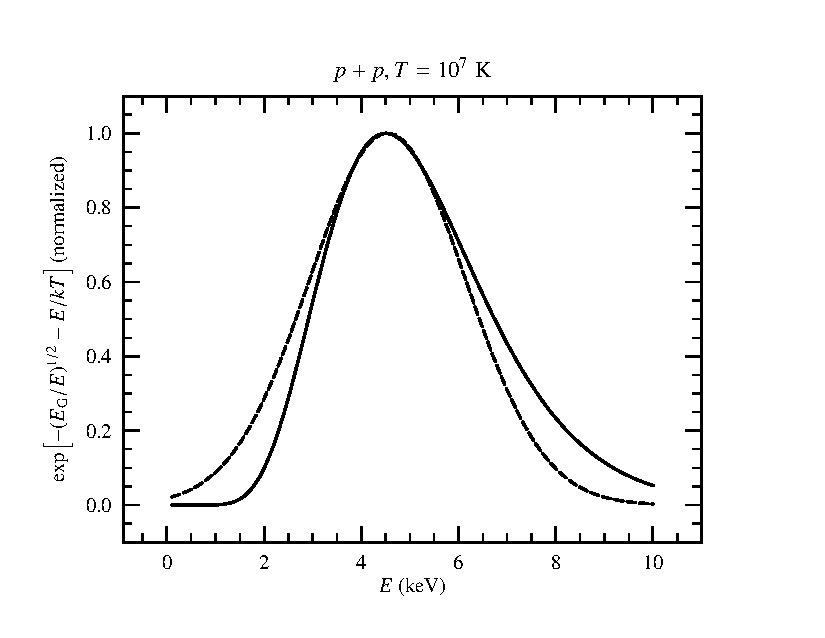
\includegraphics[width=4in]{plots_out/coulomb_integrand}
\caption{Integrand of eq.~(\protect\ref{e.integral}) (\emph{solid line}) and the Gaussian (\emph{dashed line}) constructed by expanding to second order the argument of the exponential. The parameters for $\EG$ were taken from the $p+p$ reactions ($Z_{1}Z_{2}=1$, $A = 1/2$), and the temperature is $10^{7}\nsp\K$.}
\label{f.integrand}
\end{figure}

Another simplification can be made because both the Gaussian and the original integrand go to zero as $E\to 0$.  As a result, we can extend the lower bound of our integral (eq.~[\ref{e.integral2}]) to $-\infty$, and obtain
\begin{eqnarray}\label{e.rate2}
\langle\sigma v\rangle &\approx& \left(\frac{8}{\pi m}\right)^{1/2}\left(\frac{1}{kT}\right)^{3/2} S(\Epk) \exp\left[-3\left(\frac{\EG}{4kT}\right)^{1/3}\right]\frac{\Delta}{2}\nonumber\\
 &=& \frac{2^{13/6}}{\sqrt{3m}}\frac{\EG^{1/6}}{(kT)^{2/3}} \exp\left[-3\left(\frac{\EG}{4kT}\right)^{1/3}\right]  S(\Epk).
\end{eqnarray}
On to some numbers. Table~\ref{t.reaction} lists quantities for some common reactions. A couple of notes. First, $\Delta/\Epk$ indicates how well our Gaussian approximation works---you will see it is less than 1 in all cases. We evaluated $\Delta/\Epk$, which decreases with temperature as $T^{-1/6}$, at $T = 10^{7}\nsp\K$. Second, the quantity $n(T)$ is the exponent if we want to approximate the reaction rate as a power-law, $r\propto T^{n}$.  We compute this as 
\begin{equation}\label{e.exponent}
 n(T) = \frac{\dif\ln r}{\dif\ln T} = -\frac{2}{3} + \left(\frac{\EG}{4kT}\right)^{1/3},
 \end{equation}
 as you can easily verify for yourself. In the table, the exponent is evaluated at $T = 10^{7}\nsp\K$; obviously $n$ depends on temperature. Finally, note the size of $\EG/(4k)$.  This makes the argument of the exponential in equation~(\ref{e.rate2}) large in absolute value, and sets the temperature scale at which a given reaction comes into play.
 
\begin{table}[htbp]
\caption{\label{t.reaction} Parameters for non-resonant reactions}
\centering
\begin{tabular}{lrrrrrr}
\hline
Reaction & $p+p$ & $p+\helium[3]$ & $\helium[3]+\helium[3]$ & $p+\lithium[7]$ & $p+\carbon$\\
\hline\hline
$A$ & 1/2 & 3/4 & 3/2 & 0.88 & 0.92 \\
$Z_{1}Z_{2}$ & 1 & 1 & 4 & 3 & 6 \\
$\EG$ (MeV) & 0.489 & $2.94$ & $23.5$ & $7.70$ & $32.5$\\
$\EG/(4k)$ (GK) & $1.4$ & $8.5$ & $68.0$ & $22.0$ & $94.0$ \\
$\Epk|_{T=10^{7}\nsp\K}$ (keV) & 4.5 & 8.2 & 16.3 & 11.3 & 18.2\\
$\Delta/\Epk|_{T=10^{7}\nsp\K}$ & 1.0 & 0.75 & 0.53 & 0.64 & 0.50 \\
$n(T = 10^{7}\nsp\K)$ & 4.6 & 8.8 & 18.3 & 12.4 & 20.5\\
\hline
\end{tabular}
\end{table}

\section{Exercises}

\begin{enumerate}
\item 
\begin{enumerate}
\item For a fixed $A$, what is the $Z_\star(A)$ such that the binding energy per nucleon, $f = B(N,Z)/A$ is maximized?  
\item\label{p.one} Plot $Z_{\star}$ vs $N$.
\item Using this $Z_{\star}$, plot $Y_{e}=Z_{\star}/A$ for $4 < A < 200$ and explain qualitatively any trends.
\item Now substitute the value of $Z_{\star}$ into the expression for $B(N,Z)$ and plot $B(N,Z_{\star})$ as a function of $A = N + Z_{\star}$. Explain qualitatively any trends.
\end{enumerate}
\item
\begin{enumerate}
\item\label{p.two} For each $2\le Z\le 82$, find the maximum value of $N$ such that $S_{n}(N,Z) > 0$.  Plot the values $(N,Z)$ you find.  
\item\label{p.three} For each $2\le N\le 120$, find the maximum value of $Z$ such that $S_{p}(N,Z) > 0$. Plot the values $(N,Z)$ you find. 
\end{enumerate}

\item Compare the plots of problems \ref{p.one}, \ref{p.two}, and \ref{p.three} to a chart of the nuclides.

\item In the r-process, a heavy seed nucleus captures a large number of neutrons and then decays back to stability.  Suppose we start with \iron[56] in a bath of free neutrons, so that the iron nucleus captures 152 neutrons (with $\beta$-decays occurring as necessary to keep the nucleus bound) until it reaches the stable nucleus \lead[208].  Is this process exothermic or endothermic? Explain your answer.

\item Compute the mass of H, in units of solar masses, that must be converted into \helium\ in order to supply the solar luminosity over $10^{10}\nsp\yr$.
\end{enumerate}

 